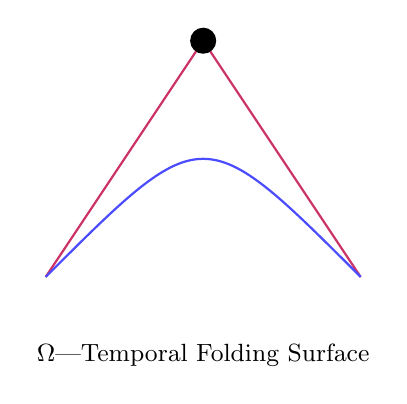
\begin{tikzpicture}[
    fold/.style={thick, draw=blue!70},
    curve/.style={thick, draw=purple!80}
]

% Light cone
\draw[curve] (0,0) -- (-2,-3);
\draw[curve] (0,0) -- (2,-3);

% Folded surface
\draw[fold] (-2,-3)..controls(0,-1)..(2,-3);

\node[circle,fill=black,minimum size=6pt] at (0,0) {};

\node at (0,-4) {\small $\Omega$---Temporal Folding Surface};

\end{tikzpicture}